\documentclass[conference, 10pt]{IEEEtran}
% \IEEEoverridecommandlockouts
% The preceding line is only needed to identify funding in the first footnote. If that is unneeded, please comment it out.
\usepackage{cite}
\usepackage{amsmath,amssymb,amsfonts}
\usepackage{algorithmic}
\usepackage{graphicx}
\usepackage{textcomp}
\usepackage{xcolor}
\usepackage{float}
\begin{document}

\title{Time Series Forecasting using Recurrent Neural Networks}

\author{\IEEEauthorblockN{Schalk Visagie}
\IEEEauthorblockA{\textit{Computer Science Department} \\
\textit{Stellenbosch University}\\
Stellenbosch, South Africa \\
25349589@sun.ac.za}
}

\maketitle

\begin{abstract}
    Time series forecasting is a critical task for which Recurrent Neural Networks (RNNs) are well-suited due to their
    ability to model sequential data. Foundational architectures such as the Elman-RNN and the Jordan-RNN offer distinct
    approaches to capturing temporal dependencies. This paper conducts a comparison of the Elman-RNN, Jordan-RNN, and a
    hybrid Multi-Recurrent Neural Network (MRNN) to determine if a superior architecture emerges for time series
    forecasting in a given dataset. The evaluation is performed on five datasets with diverse characteristics: a
    synthetic autoregressive series, S\&P 500 and VIX financial indices, an electricity load profile, and a multivariate
    weather series. For each model and dataset, a comprehensive hyperparameter search is conducted using a
    growing-window cross-validation strategy to ensure a fair comparison. The final performance, measured by Root Mean
    Squared Error (RMSE) and Mean Absolute Error (MAE) on a holdout test set, reveals that all three architectures
    achieve remarkably similar predictive accuracy. Despite their structural differences, no single model demonstrated a
    consistent or significant advantage across the varied forecasting tasks. This suggests that the specific choice
    between these foundational RNN feedback mechanisms may be less critical to forecasting performance than robust
    hyperparameter tuning and appropriate data preprocessing.
\end{abstract}

% \begin{IEEEkeywords}

% \end{IEEEkeywords}

\section{Introduction}

Time series forecasting is a critical task in many domains, involving the prediction of future values based on
historical data. RNNs are a class of neural networks specifically designed for sequential
data, making them highly suitable for such forecasting tasks. The defining feature of RNNs is the presence of feedback
loops, which allow the networks to maintain an internal state or memory of past information to influence future
predictions.

Among the foundational RNN architectures are the Elman-RNN and the Jordan-RNN. The Elman-RNN captures temporal dynamics
by feeding the previous hidden state back into the current hidden layer computation. In contrast, the Jordan-RNN
utilizes feedback from the network's previous output to inform the current hidden state. The MRNN is a hybrid
architecture that integrates both of these feedback mechanisms, theoretically enabling the capture of more complex
temporal dependencies.

While these three architectures are well-established, a direct and rigorous comparison of their performance across
diverse time series problems is necessary to guide model selection. This paper aims to fill that gap by evaluating the
predictive capabilities of the Elman-RNN, Jordan-RNN, and MRNN. The primary objective is to determine which architecture
provides the most accurate forecasts across datasets with varying characteristics, such as stationarity, seasonality,
and multivariate dependencies.

The comparative analysis is conducted using five distinct datasets: a synthetic autoregressive series, the S\&P 500 and
VIX financial indices, an electricity load profile, and a multivariate weather dataset. To ensure a fair and robust
evaluation, a comprehensive hyperparameter tuning process is implemented for each model on each dataset using a
growing-window cross-validation strategy, which respects the temporal order of the data. The final performance of the
optimized models is then assessed on an unseen holdout test set, using RMSE and MAE as the primary evaluation metrics.

The remainder of this paper details this investigation. The background section provides a technical overview of the
three RNN architectures and their training process. The methodology section describes the datasets, the cross-validation
procedure, and the measures taken to prevent overfitting. Following this, the empirical procedure outlines the
experimental setup and hyperparameter tuning framework. The results section presents the performance of each model on
the holdout test sets, leading to a final conclusion on the relative strengths of the Elman-RNN, Jordan-RNN, and MRNN
for time series forecasting.


\section{Background}

The notation used in the equations for the RNN architectures is defined as follows. The term $h_t$ represents the hidden
state vector at the current time step $t$. The input to the network at the same time step is given by the vector $X_t$.
The feedback mechanisms rely on information from the previous time step, where $h_{t-1}$ is the hidden state and
$y_{t-1}$ is the network's output. The network's learnable parameters include the weight matrices and a bias vector.
Specifically, $W_{xh}$ is the weight matrix connecting the input layer to the hidden layer, $W_{hh}$ is the recurrent
weight matrix from the previous hidden state to the current hidden state, and $W_{yh}$ is the weight matrix from the
previous output to the hidden state. The term $b_h$ represents the bias vector for the hidden layer. Finally, $\tanh$
denotes the hyperbolic tangent activation function.

\textbf{Elman Recurrent Neural Network }

The Elman-RNN is a simple RNN architecture consisting of an input layer, a hidden layer, a context layer, and an output
layer. The context layer, with the same number of neurons as the hidden layer, stores a copy of the previous hidden
state and feeds it back to the hidden layer, enabling the network to maintain short-term memory of past inputs. The
Elman-RNN hidden state is computed as follows:
$$h_t = \tanh(W_{xh}X_t + W_{hh}h_{t-1} + b_h)$$
% TODO: add explaination of the notation

This feedback loop introduces temporal dynamics, distinguishing it from feedforward
networks.

Elman-RNN is suitable for time series prediction because its recurrent structure captures sequential dependencies,
allowing it to model patterns in data where current values depend on historical context, such as a simple sequence of
XOR operations, stock prices or weather.

\textbf{Jordan Recurrent Neural Network }

The Jordan recurrent neural network (Jordan-RNN) features an input layer, hidden layer, context layer, and output layer. Unlike
Elman-RNN, the context layer stores previous output values and feeds them back to the hidden layer, creating a feedback
loop from outputs to influence future computations. The Jordan-RNN hidden states are computed as:

$$h_t = \tanh(W_{xh}X_t + W_{yh}y_{t-1} + b_h)$$

The Jordan-RNN's context layer has the same number of neurons as its output layer in contrast to the Elman-RNN having a
context layer with the same size as its hidden layer.

Jordan-RNN applies to time series prediction by leveraging output feedback to handle temporal correlations, making it
effective for forecasting tasks like price trends where past predictions inform future ones.

\textbf{Multi-Recurrent Neural Network }

The multi-recurrent neural network (MRNN) integrates features of both Elman-RNN and Jordan-RNN. It includes input,
hidden, context, and output layers. The context layer receives feedback from both previous hidden states and
outputs and presented to the hidden layer at each time step. This hybrid architecture enhances memory by combining multiple
recurrent paths. The MRNN hidden states are computed by the following equation: 

$$h_t = \tanh(W_{xh}X_t + W_{hh}h_{t-1} + W_{yh}y_{t-1} + b_h)$$

MRNN is apt for time series prediction as its dual feedback mechanisms provide an alternative way to capture complex
temporal dependencies in sequential data compared to the previous two single-loop variants.

While specific equations vary, MRNN extends Elman-RNN and Jordan-RNN formulations by incorporating both hidden and
output feedbacks in the hidden state computation, such as combining terms from \( h(t-1) \) and \( y(t-1) \) in the
activation.

\textbf{Backpropagation Training Process} 

The training process relies on backpropagation through time (BPTT) to effectively manage the sequential nature of the
data. This method works by unfolding the recurrent network across multiple time steps, essentially converting it into a
layered feedforward network where the weights are shared among the time-unfolded layers, allowing the use of standard
backpropagation techniques to calculate gradients \cite{quarkmlBackpropagationThrough}.

The process starts with a forward pass through the network. For each time step $t$ in the sequence, the hidden state is
calculated as \( h_t = \tanh(W_{xh} \cdot X_t + W_{hh} \cdot h_{t-1} + b_h) \), where \( X_t \) represents the input at
that step, \( W_{xh} \) is the weight matrix from input to hidden, \( W_{hh} \) is the recurrent weight matrix from
previous hidden to current hidden, and \( b_h \) is the hidden bias. Following this, the output at each time step is
computed as \( y_t = \phi(W_{oh} \cdot h_t + b_o) \), with \( W_{oh} \) as the weight matrix from hidden to output, \(
b_o \) as the output bias, tanh as the activation for the hidden layer, and \( \phi \) (such as sigmoid or softmax) for
the output layer \cite{quarkmlBackpropagationThrough}.

Next, the loss is evaluated, often using mean squared error for regression tasks like time series prediction: \( L =
\frac{1}{N} \sum_{t=1}^{N} (y - y_t)^2 \), where y is the target value and N is the number of time steps. The derivative
of this loss with respect to the predicted output is \( \frac{\partial{L}}{\partial{y_t}} = \frac{2}{n}\sum_{t=t}^{n}(y
- y_t) \) providing the starting point for error propagation.

The backward pass then proceeds by applying the chain rule to propagate errors back through the unfolded network,
accumulating gradients over all time steps. For the output weights, the gradient is \( \frac{\partial L}{\partial
W_{oh}} = \sum_{i=0}^{t} \frac{\partial L}{\partial y_{t-i}} \cdot \frac{\partial y_{t-i}}{\partial W_{oh}} \), which
sums contributions from each relevant time step. For the input-to-hidden weights, it is \( \frac{\partial L}{\partial
W_{xh}} = \sum_{i=0}^{t} \left[ \left( \frac{\partial L}{\partial y_{t-i}} \cdot \frac{\partial y_{t-i}}{\partial
h_{t-i}} \right) \cdot \left( \prod_{j=(t-i+1)}^{t} \frac{\partial h_j}{\partial h_{j-1}} \right) \cdot \frac{\partial
h_{t-i}}{\partial W_{xh}} \right] \), accounting for how errors flow through the recurrent connections. Similarly, for
the hidden-to-hidden weights: \( \frac{\partial L}{\partial W_{hh}} = \sum_{i=0}^{t} \left[ \left( \frac{\partial
L}{\partial y_{t-i}} \cdot \frac{\partial y_{t-i}}{\partial h_{t-i}} \right) \cdot \left( \prod_{j=(t-i+1)}^{t}
\frac{\partial h_j}{\partial h_{j-1}} \right) \cdot \frac{\partial h_{t-i}}{\partial W_{hh}} \right] \). 

Once these gradients are computed, the weights are updated using gradient descent with a learning rate \( \alpha \).
Care must be taken with long sequences to mitigate issues like vanishing or exploding gradients that can arise from
repeated multiplications in the product terms \cite{quarkmlBackpropagationThrough}.

In the context of specific architectures, BPTT in Elman-RNNs emphasizes updating the hidden-to-context feedback to
capture internal dynamics; in Jordan-RNNs, it prioritizes the output-to-context loop for incorporating prior
predictions; and in MRNN, it handles both types of feedback simultaneously.

\textbf{Adam Optimization Algorithm}
The Adam (Adaptive Moment Estimation) optimizer is a widely used algorithm for stochastic gradient-based optimization in
machine learning, particularly effective for training simple RNNs on time series data. It adapts the learning rate for
each parameter by computing exponentially decaying averages of past gradients and past squared gradients, combining
ideas from Root Mean Square Propagation and momentum methods. This adaptive approach helps in handling sparse gradients
and non-stationary objectives, leading to faster convergence and better performance in noisy environments
\cite{kingma2017adammethodstochasticoptimization} \cite{machinelearningmasteryGentleIntroduction}.

Adam integrates with backpropagation by using the gradients computed through backpropagation to update the model's
parameters in an adaptive manner during RNN training. Backpropagation calculates the error gradients by propagating the
loss backward through the unrolled RNN over time steps, addressing issues like vanishing gradients in recurrent
structures. Adam then applies these gradients to its moment estimates, adjusting learning rates per parameter to
optimize weight updates, which enhances convergence speed and stability for time series prediction tasks in shallow RNNs \cite{machinelearningmasteryGentleIntroduction}.

\section{Methodology}
\subsection{Dataset descriptions}

\textbf{S\&P 500 ETF Daily OHLCV} dataset was obtained from Yahoo Finance. This dataset comprises 5,031 trading days of
Open, High, Low, Close, and Volume data from 19 September 2005 to 19 September 2025. This dataset is particularly
relevant for evaluating RNN architectures due to its inherent non-stationarity, inconsistent variance, and complex
non-linear dependencies, which provide a robust benchmark for comparing the ability of different models to learn
patterns in time series data and predict next-step closing price. Preprocessing was necessary to ensure data quality and
model stability. The 85 instances identified as outliers in the training data set ($\sigma >$ 3) were clamp-transformed
to 3 standard deviations from the mean. The closing price, confirmed as non-stationary by Augmented Dickey-Fuller (ADF)
and Kwiatkowski-Phillips-Schmidt-Shin (KPSS) tests, was stabilized by conversion to log returns
\cite{StationarityTests}.\\

$log\_return_t = log(close_t / close_{t-1})$\\

Using log returns is a common way to make financial time series data stationary. Log returns were the only feature used
in this dataset Feature scaling for all datasets is discussed in subsection C along with the time series cross
validation.

\textbf{CBOE VIX Daily OHLC} dataset, sourced from Yahoo Finance, provides 5,031 observations of daily Open, High, Low,
and Close data for the period spanning 19 September 2005 to 19 September 2025. This time series is well-suited for
testing RNNs because its structural properties. These structural properties include sudden spikes, and shifting
sequential dependencies that create challenging non-stationary patterns. These characteristics differ significantly from
the other datasets which make it an ideal candidate for diversifying training data. Data preparation involved several
steps. First, 73 outliers in the training set exceeding 3 standard deviations were clamped. The non-stationarity of the
closing price, verified with ADF and KPSS tests, was resolved by transforming the series' Close feature into log
returns. Similar to the S\&P 500 data. Log returns was once again the only feature used for training the models in this
dataset.

The \textbf{ElectricityLoadDiagrams20112014} dataset contains high-frequency electricity consumption readings in
kilowatts for 370 clients, recorded every 15 minutes from January 2011 to the end of 2014. For this assignment, a single
client's consumption profile, consisting of 140,256 measurements, was arbitrarily selected to create a univariate time
series forecasting scenario. This dataset was reduced to a size of 15000 measurements by only using the first few
observations. This was done to reduce model training and hyperparameter tuning time to be reasonable. This provides a
high-granularity, cyclical test case for evaluating the predictive performance of the RNN models. The data required
minimal cleaning as it contained no missing values. However, power consumption values in the training set exceeding 3
standard deviations from the mean were clamp-transformed to handle outliers. Both ADF and KPSS tests confirmed that the
series was non-stationary. To address this, a 24-hour seasonal differencing was applied, accounting for the inherent
daily cyclicality of energy usage.

The \textbf{Synthetic Autoregressive Stationary (AR(1))} dataset was generated using Python code with the \texttt{NumPy}
library, simulating a univariate time series from an AR(1) process defined by the equation $x_t = 0.5 x_{t-1} +
\epsilon_t$, where $\epsilon_t$ is white noise drawn from a normal distribution with mean 0 and standard deviation 1.
This dataset consists of 2000 sequential observations, following a 500-point burn-in period to ensure the process reaches
stationarity. It is particularly suitable for benchmarking RNN architectures in this project due to its inherent
stationarity, linear autoregressive dependencies, and absence of trends or seasonality, offering a controlled
environment to evaluate the models' ability to capture simple recurrent patterns without the confounding factors present
in real-world data, thereby serving as a baseline for comparison with non-stationary datasets. The synthetic nature
ensured no missing values or structural anomalies. Stationary was confirmed both by design (autoregressive coefficient
$|\phi| = 0.5 < 1$) and through ADF and KPSS tests.

The \textbf{TimeSeries Weather Dataset}, sourced from Kaggle, contains hourly historical weather data for two locations.
The location having more records (389,496 observations spanning January 1, 1980, to June 6, 2024) was selected. This
dataset is a multivariate time series with 17 continuous features, including temperature, humidity, dew point,
precipitation, pressure and cloud cover to name a few. This dataset was chosen for its high temporal granularity,
pronounced daily and seasonal cycles as well as multivariate interactions. Its inclusion enhances dataset diversity by
introducing time series data with multiple cyclical tendencies and non-stationarity, contrasting the previously
mentioned datasets. The data exhibited no missing values or major irregularities. Outliers exceeding 3 standard
deviations were clamp-transformed. Highly correlated features with absolute correlation greater than 0.75 were dropped
to reduce multicollinearity while preserving predictive power. The target feature is defined as the next hour's
differenced temperature. Non-stationarity, confirmed by ADF and KPSS tests, was addressed through 24-hour seasonal
differencing to account for daily periodicity.

\subsection{Recurrent Neural Networks Implemented}
Elman, Jordan and MRNNs were implemented exactly as outlined in the background section. For each dataset the
models were trained using the Adam optimization algorithm that uses gradients computed via BPTT. The key hyperparameters
for the Adam optimizer, namely the learning rate and weight decay were determined through hyperparameter tuning.

The Mean Squared Error (MSE) was employed as the loss function to guide the training process. MSE is a standard choice
for regression tasks, as it measures the average squared difference between the predicted values ($\hat{y}$) and the actual
values ($y$). It is defined by the formula:

$$L_{MSE} = \frac{1}{N} \sum_{i=1}^{N} (y_i - \hat{y}_i)^2$$ 

This function is differentiable and penalizes larger prediction errors more heavily, making it effective for model
optimization.

\subsection{Cross Validation Implementation}
To tune hyperparameters and assess model performance, a growing-window cross-validation procedure was implemented as
described in \cite{CrossValidationTimeseries}. Standard $k$-fold cross-validation is inappropriate for time series data
because it shuffles observations, thereby destroying their temporal order \cite{CrossValidationTimeseries}.

The growing-window approach respects this temporal structure. The process begins by training the model on an initial,
chronological segment of the data and validating it on the immediately following block of data. In each subsequent fold,
the training set is expanded to include the data from the previous validation block, while the next sequential block is
used for validation. This method simulates a realistic forecasting scenario where a model is periodically retrained as
new data becomes available, ensuring that the model is always validated on "future" data relative to its training set.
For each fold, the training data was standardized using scikit-learn's \texttt{StandardScaler()}, which removes the mean
and scales features to unit variance. The corresponding validation fold was transformed using the scaler fitted on its
respective training data. This procedure ensures that the scaling parameters are derived exclusively from the training
set, thereby preventing any information leakage from the validation set. As a result, the validation data is transformed
using the statistics of the training data, maintaining the integrity of the evaluation and reflecting a realistic
forecasting scenario.

\subsection{Overfitting/Underfitting Prevention}
A multi-faceted strategy was implemented to ensure the models achieved a balance between underfitting and overfitting.

To prevent underfitting, a \textbf{grid search} was conducted over a range of hyperparameters, including the number of hidden
units, sequence length, weight decay, early stopping and learning rate. This systematic exploration ensures that the
final model has sufficient complexity and capacity to capture the underlying patterns present in the data.

To prevent overfitting, two distinct regularization techniques were applied during training:

\textbf{Weight Decay (L2 Regularization):} This was incorporated directly into the Adam optimizer. By adding a penalty term to
the loss function proportional to the squared magnitude of the model weights, this technique discourages the learning of
overly complex models that might fit the noise in the training data.

\textbf{Early Stopping:} The model's performance on the validation set of each fold was measured at the end of every epoch. If
the validation loss did not show improvement for a predefined number of epochs (the patience parameter), the training
process was halted. This prevents the model from continuing to train once starts to overfit the training data.

\section{Empirical Procedure}
This section details the systematic process used to train, tune, and evaluate the Elman-RNN, Jordan-RNN, and MRNNs across all
five datasets. The procedure is designed to ensure reproducibility and a fair comparison between the models.

\subsection{Experimental setup}
The experiments were conducted using the \texttt{PyTorch} library for neural network implementation, supplemented by \texttt{scikit-learn}
for data scaling and \texttt{pandas} for data management. To ensure reproducibility, the random seeds for both \texttt{NumPy} and \texttt{PyTorch}
were fixed to a constant value of 42.

For each dataset, a chronological data partitioning strategy was employed. The data was first split into a 70\%
training/validation set and a 30\% holdout test set. The holdout set was strictly used only for a single final evaluation
of the optimized models to provide an unbiased assessment of generalization performance.

Model performance was evaluated using Root Mean Squared Error (RMSE) and Mean Absolute Error (MAE). During the
hyperparameter tuning phase, the mean RMSE across cross-validation folds served as the primary metric for hyperparameter
selection. Final performance on the holdout set was reported in terms of RMSE on both the scaled data and the
inverse-transformed, original scale of the data for better interpretability.

\subsection{Hyperparameter Tuning}
A comprehensive grid search coupled with a 5-fold growing-window cross-validation was performed to identify the optimal
hyperparameters for each of the three RNN architectures on each dataset.

The hyperparameter search space was defined as follows:

\begin{itemize}
    \item \textbf{Hidden Layer Size:} [32, 64, 96]
    \item \textbf{Learning Rate:} [0.00001, 0.0001, 0.0005, 0.001]
    \item \textbf{Sequence Length:} [10, 25]
    \item \textbf{Weight Decay:} [1e-5, 1e-4, 1e-3]
    \item \textbf{Early Stopping Patience:} [10, 15, 20] epochs
\end{itemize}

Throughout all experiments, several architectural and training parameters were held constant to ensure a controlled
comparison. These included the Adam optimizer, Mean Squared Error (MSE) loss function, a single recurrent layer, a batch
size of 32, and a \texttt{tanh} hidden layer activation function. Training was conducted for a maximum of 100 epochs,
with early stopping implemented to prevent overfitting.

The described grid search's results are included in the appendix Table \ref{hyperparameters}

\subsection{Final Training and Evaluation}

The final evaluation followed three steps. First, the hyperparameter combination that achieved the lowest average RMSE
during the growing-window cross-validation was identified for each RNN model. Second, a new model was made with these
optimal hyperparameters and retrained from scratch on the entire 70\% training dataset. Finally, this fully trained
model was evaluated one time on the unseen 30\% holdout test set to measure its definitive performance. Do note that
plots presented in this section are made using the inversely transformed stationary versions of the datasets

\subsection{Model Comparison Framework}
To determine the best-performing RNN architecture for each dataset, the final holdout set RMSE and MAE scores from the
three optimized models (Elman, Jordan, and MRNN) were directly compared. The architecture yielding the lowest error
on the holdout data was concluded to be the most effective for that particular time series. This complete empirical
procedure was consistently repeated for all five datasets, providing a standardized basis for the final results and
conclusions.

\section{Results}
Results This section presents the empirical results obtained from evaluating the Elman, Jordan, and MRNN on the five
selected time series datasets. The results are derived from the empirical procedure outlined in the previous section,
utilizing the optimal hyperparameters identified via grid search and growing-window cross-validation. Performance is
reported in terms of Root Mean Squared Error (RMSE) and Mean Absolute Error (MAE) on the 30\% holdout test set, computed
both on the scaled data (for model-internal consistency) and the inverse-transformed original scale (for practical
interpretability).

For each dataset, the optimal hyperparameters are summarized, followed by a comparison of the three models. The
best-performing model per dataset is highlighted based on the lowest holdout RMSE.

\subsection{Synthetic Autoregressive Stationary Dataset}

The synthetic AR(1) dataset served as a baseline to validate the models' ability to learn simple, linear temporal
dependencies. As shown in Table \ref{tab:results_ar1}, all three architectures performed exceptionally well, achieving
nearly identical results on the holdout set. The Elman-RNN yielded a marginally lower RMSE of 1.1253, followed closely
by the Jordan-RNN and MRNN with RMSEs of 1.1254.

\begin{table}[H]
    \centering
    \begin{tabular}{|l|c|c|c|c|}
        \hline
        \textbf{Model}& \textbf{RMSE} & \textbf{MAE} \\ 
        \hline
        Elman-RNN & 1.1253 & 0.8941 \\
        \hline
        Jordan-RNN & 1.1254 & 0.8941 \\
        \hline
        MRNN & 1.1254 & 0.8943 \\
        \hline
        \textbf{Best Model} &\multicolumn{2}{c|}{{MRNN}} \\ 
        \hline
    \end{tabular}
    \vspace{4pt}
    \caption{Performance Metrics for Synthetic Autoregressive Stationary Dataset}
    \label{tab:results_ar1}
\end{table}

This performance is notable because the theoretical limit for the RMSE on this dataset is 1.0, corresponding to the
standard deviation of the white noise component ($\epsilon_t$) in the AR(1) process. An RMSE approaching this value
indicates that the models successfully captured the autoregressive signal, with the remaining error being almost
entirely due to the inherent randomness of the data. Therefore, the strong performance of these simple RNN
models confirms their capability to learn the fundamental patterns present in a stationary autoregressive time series,
establishing their suitability for tackling more complex forecasting problems.

\subsection{CBOE VIX Daily OHLC Dataset}
For the CBOE VIX dataset, characterized by its high volatility and non-stationarity, all three models again demonstrated
remarkably similar predictive accuracy. As shown in Table \ref{tab:results_vix}, the Jordan-RNN achieved a minimally
lower RMSE of 0.0787, though the differences with the Elman-RNN (0.0788) and MRNN (0.0788) are practically
insignificant. This quantitative similarity is visually confirmed in Figure \ref{fig:plots_vix}, where the forecast
plots for the three models are nearly indistinguishable.
\begin{table}[H]
    \centering
    \begin{tabular}{|l|c|c|c|c|}
        \hline
        \textbf{Model}& \textbf{RMSE} & \textbf{MAE}  \\ 
        \hline
        Elman-RNN& 0.0788 & 0.0545 \\ 
        \hline
        Jordan-RNN & 0.0787 & 0.0545  \\ 
        \hline
        MRNN & 0.0788 & 0.0545  \\ 
        \hline
        \textbf{Best Model} & \multicolumn{2}{c|}{{Jordan-RNN}} \\ 
        \hline
    \end{tabular}
    \vspace{4pt}
    \caption{Performance Metrics for CBOE VIX}
    \label{tab:results_vix}
\end{table}
The minor differences can be seen in Figure
\ref{fig:plots_vix} where the MRNN and Jordan-RNN slightly differ.

\begin{figure}[H]
    \centering
    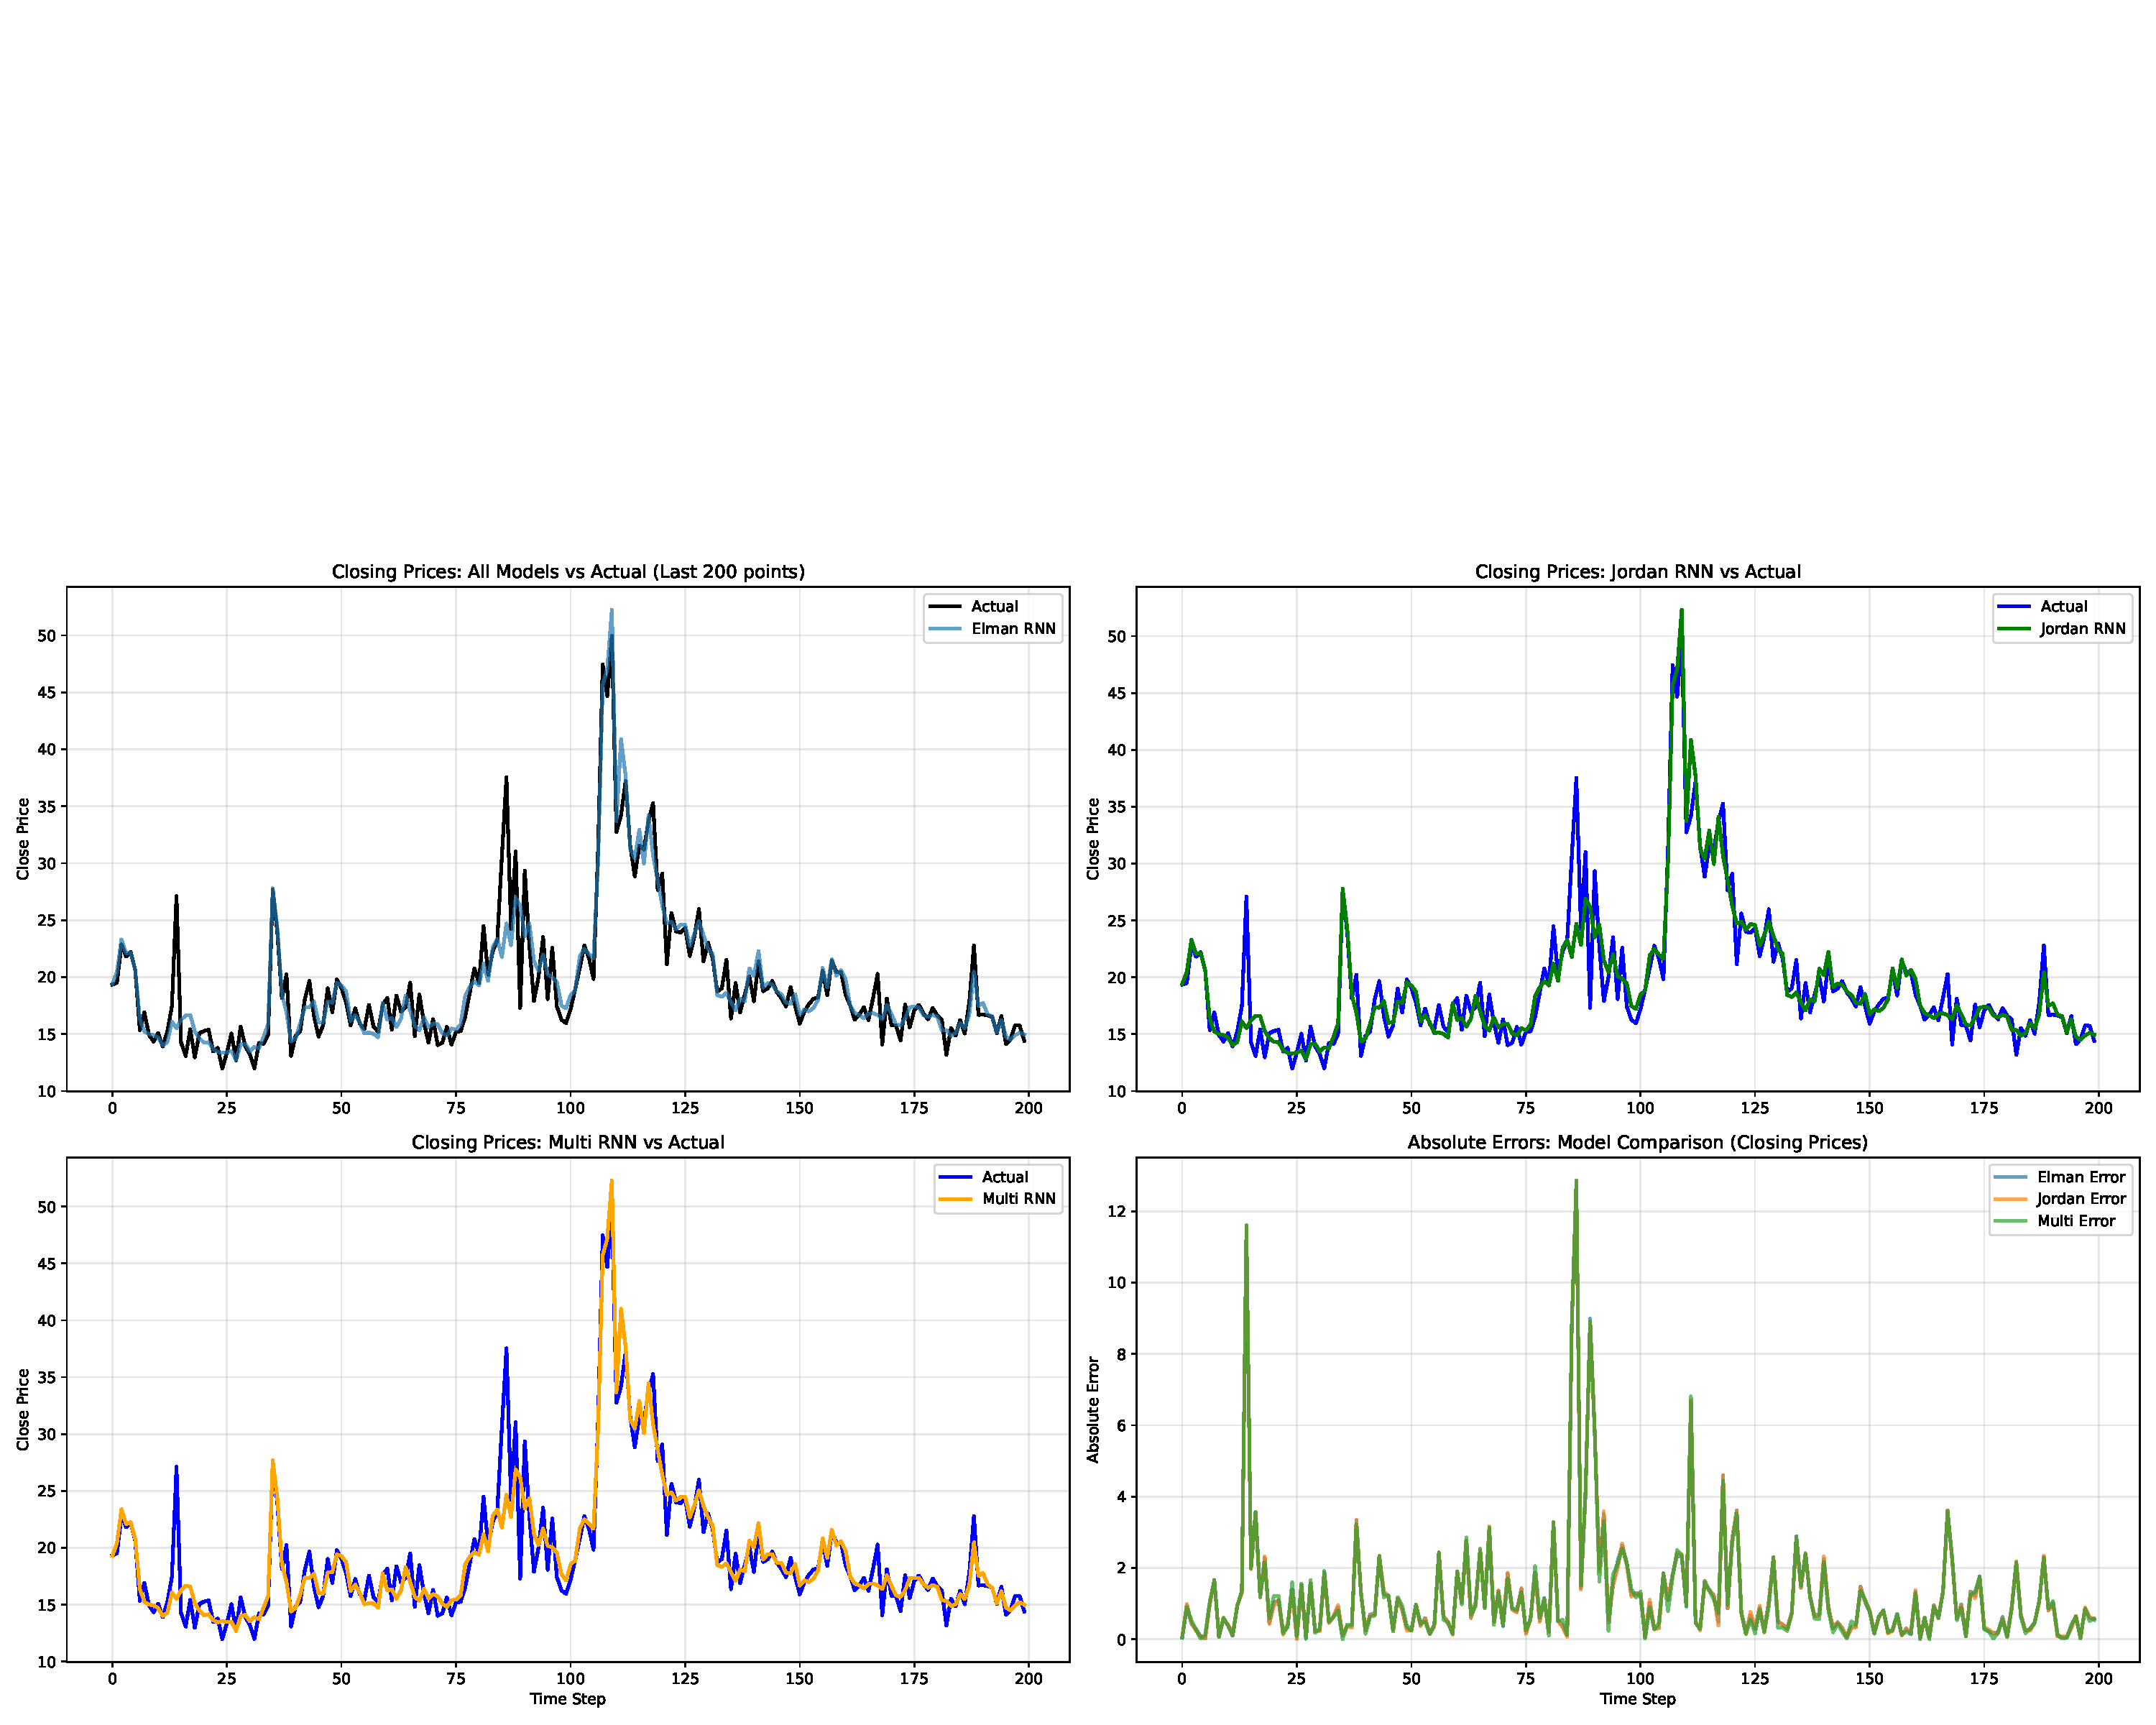
\includegraphics[width=0.5\textwidth]{plots/rnn_model_comparison_vix.pdf}
    \caption{VIX Dataset plots}
    \label{fig:plots_vix}
\end{figure}

The consistent performance on this noisy, mean-reverting financial series suggests that the simple recurrent mechanisms
of all three architectures were equally capable of modeling the complexities of this dataset. The feedback from
the previous output ($y_{t-1}$) in the Jordan-RNN did not provide a clear advantage over feedback from the internal hidden
state ($h_{t-1}$) or the hybrid approach of the MRNN.

\subsection{ElectricityLoadDiagrams20112014 Dataset}
The electricity load dataset, with its strong, high-frequency seasonality, introduced a slightly greater performance
differentiation among the models. According to the metrics in Table \ref{tab:results_elec}, the Elman-RNN emerged as the
top-performing model with an RMSE of 58.4710. The MRNN followed closely with an RMSE of 58.5584, while the Jordan-RNN
lagged slightly at 59.1565.
\begin{table}[H]
    \centering
    \begin{tabular}{|l|c|c|c|c|}
        \hline
        \textbf{Model}& \textbf{RMSE} & \textbf{MAE} \\ 
        \hline
        Elman-RNN& 58.4710 & 40.0989 \\ 
        \hline
        Jordan-RNN & 59.1565 & 40.0989 \\ 
        \hline
        MRNN &  58.5584 & 39.9769 \\ 
        \hline
        \textbf{Best Model} & \multicolumn{2}{c|}{{Elman-RNN}}\\ 
        \hline
    \end{tabular}
    \vspace{4pt}
    \caption{Performance Metrics for ElectricityLoadDiagrams20112014}
    \label{tab:results_elec}
\end{table}

Despite these numerical differences, the overall predictive power remains comparable, as illustrated by the forecast
plots in Figure \ref{fig:plots_elec}. The marginal superiority of the Elman-RNN may suggest that for time series with
highly regular internal patterns, such as daily energy consumption cycles, relying on the memory of the internal hidden
state ($h_{t-1}$) is slightly more effective for capturing the underlying structure than incorporating the potentially
noisier previous output ($y_{t-1}$).

\begin{figure}[H]
    \centering
    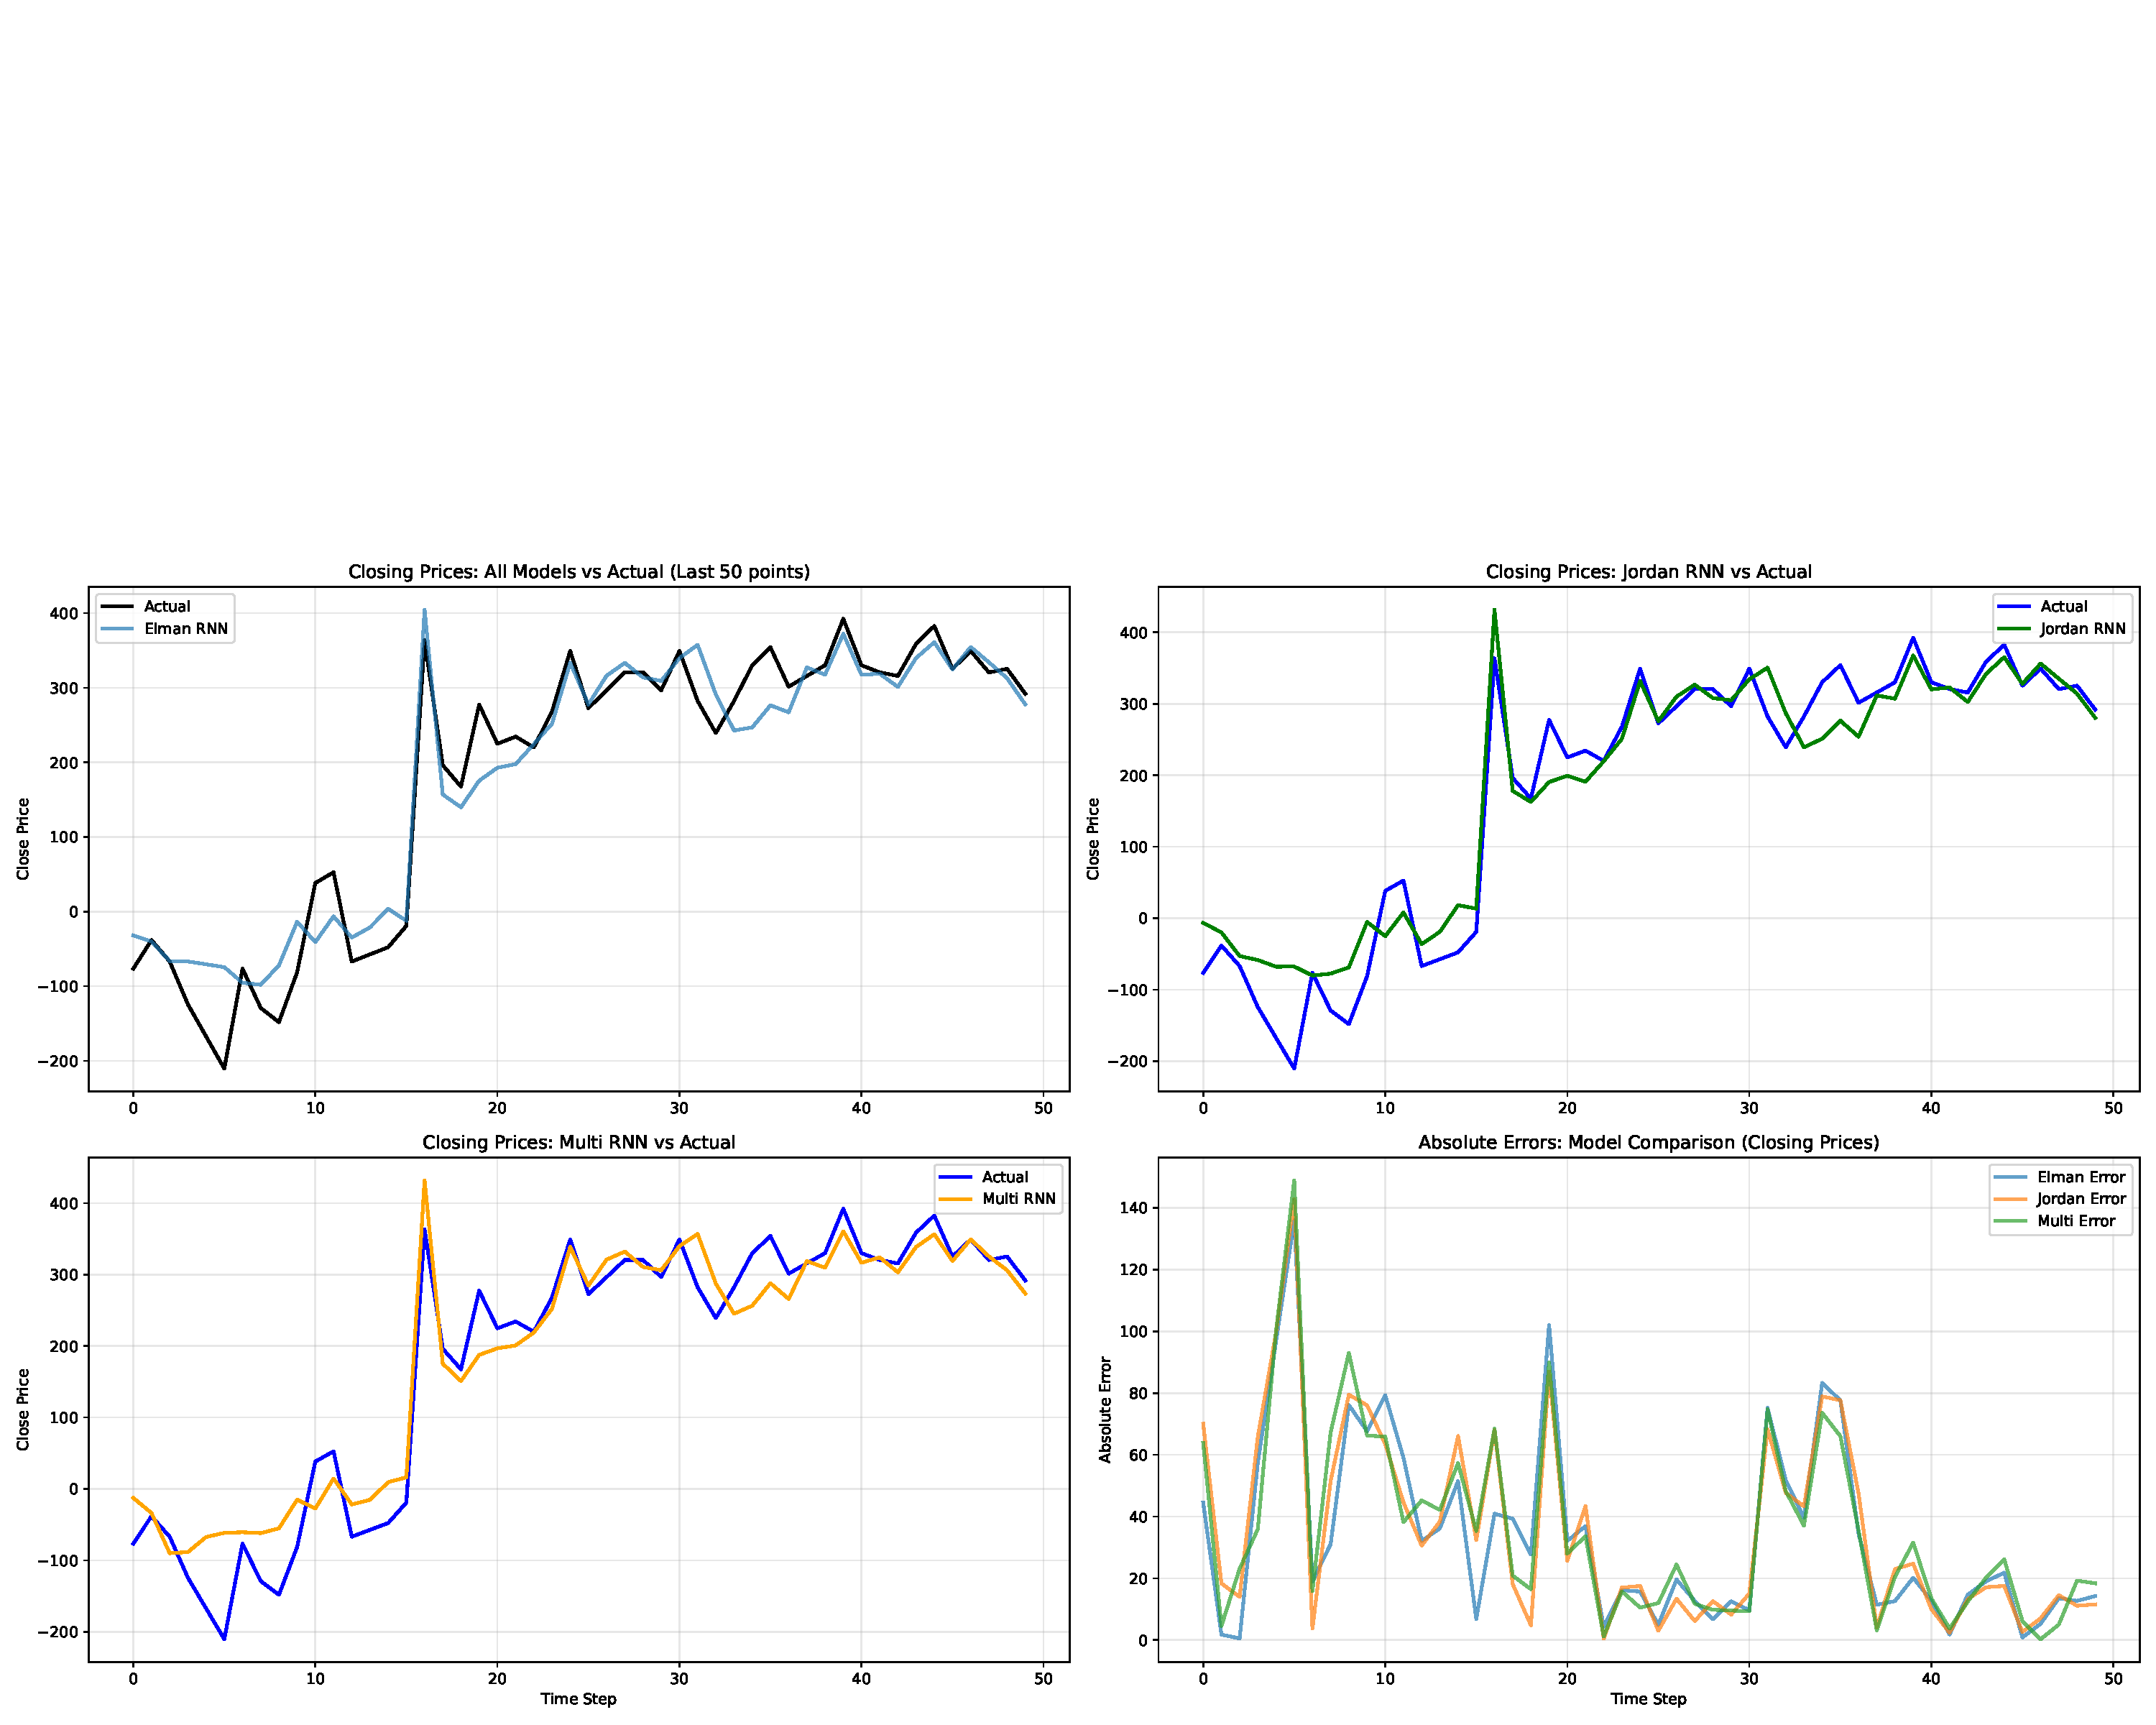
\includegraphics[width=0.5\textwidth]{plots/rnn_model_comparison_elec.pdf}
    \caption{ElectricityLoadDiagrams20112014 Dataset plots}
    \label{fig:plots_elec}
\end{figure}


\subsection{S\&P 500 ETF Daily OHLCV Dataset}
In forecasting the log returns of the S\&P 500, the models once again yielded highly comparable results. Table
\ref{tab:results_spy} shows that the Jordan-RNN obtained the lowest RMSE (0.0132), but by an extremely narrow margin
over the Elman-RNN and MRNN. 
\begin{table}[H]
    \centering
    \begin{tabular}{|l|c|c|c|c|}
        \hline
        \textbf{Model}& \textbf{RMSE} & \textbf{MAE}\\ 
        \hline
        Elman-RNN& 0.0133 & 0.0086 \\ 
        \hline
        Jordan-RNN & 0.0132 & 0.0085\\ 
        \hline
        MRNN & 0.0134 & 0.0086 \\ 
        \hline
        \textbf{Best Model} & \multicolumn{2}{c|}{{Jordan-RNN}} \\ 
        \hline
    \end{tabular}
    \vspace{4pt}
    \caption{Performance Metrics for S\&P500}
    \label{tab:results_spy}
\end{table}

The forecast plots in Figure \ref{fig:plots_spy} visually reinforce this finding, showing
that all models produce nearly identical predictions.

\begin{figure}[H]
    \centering
    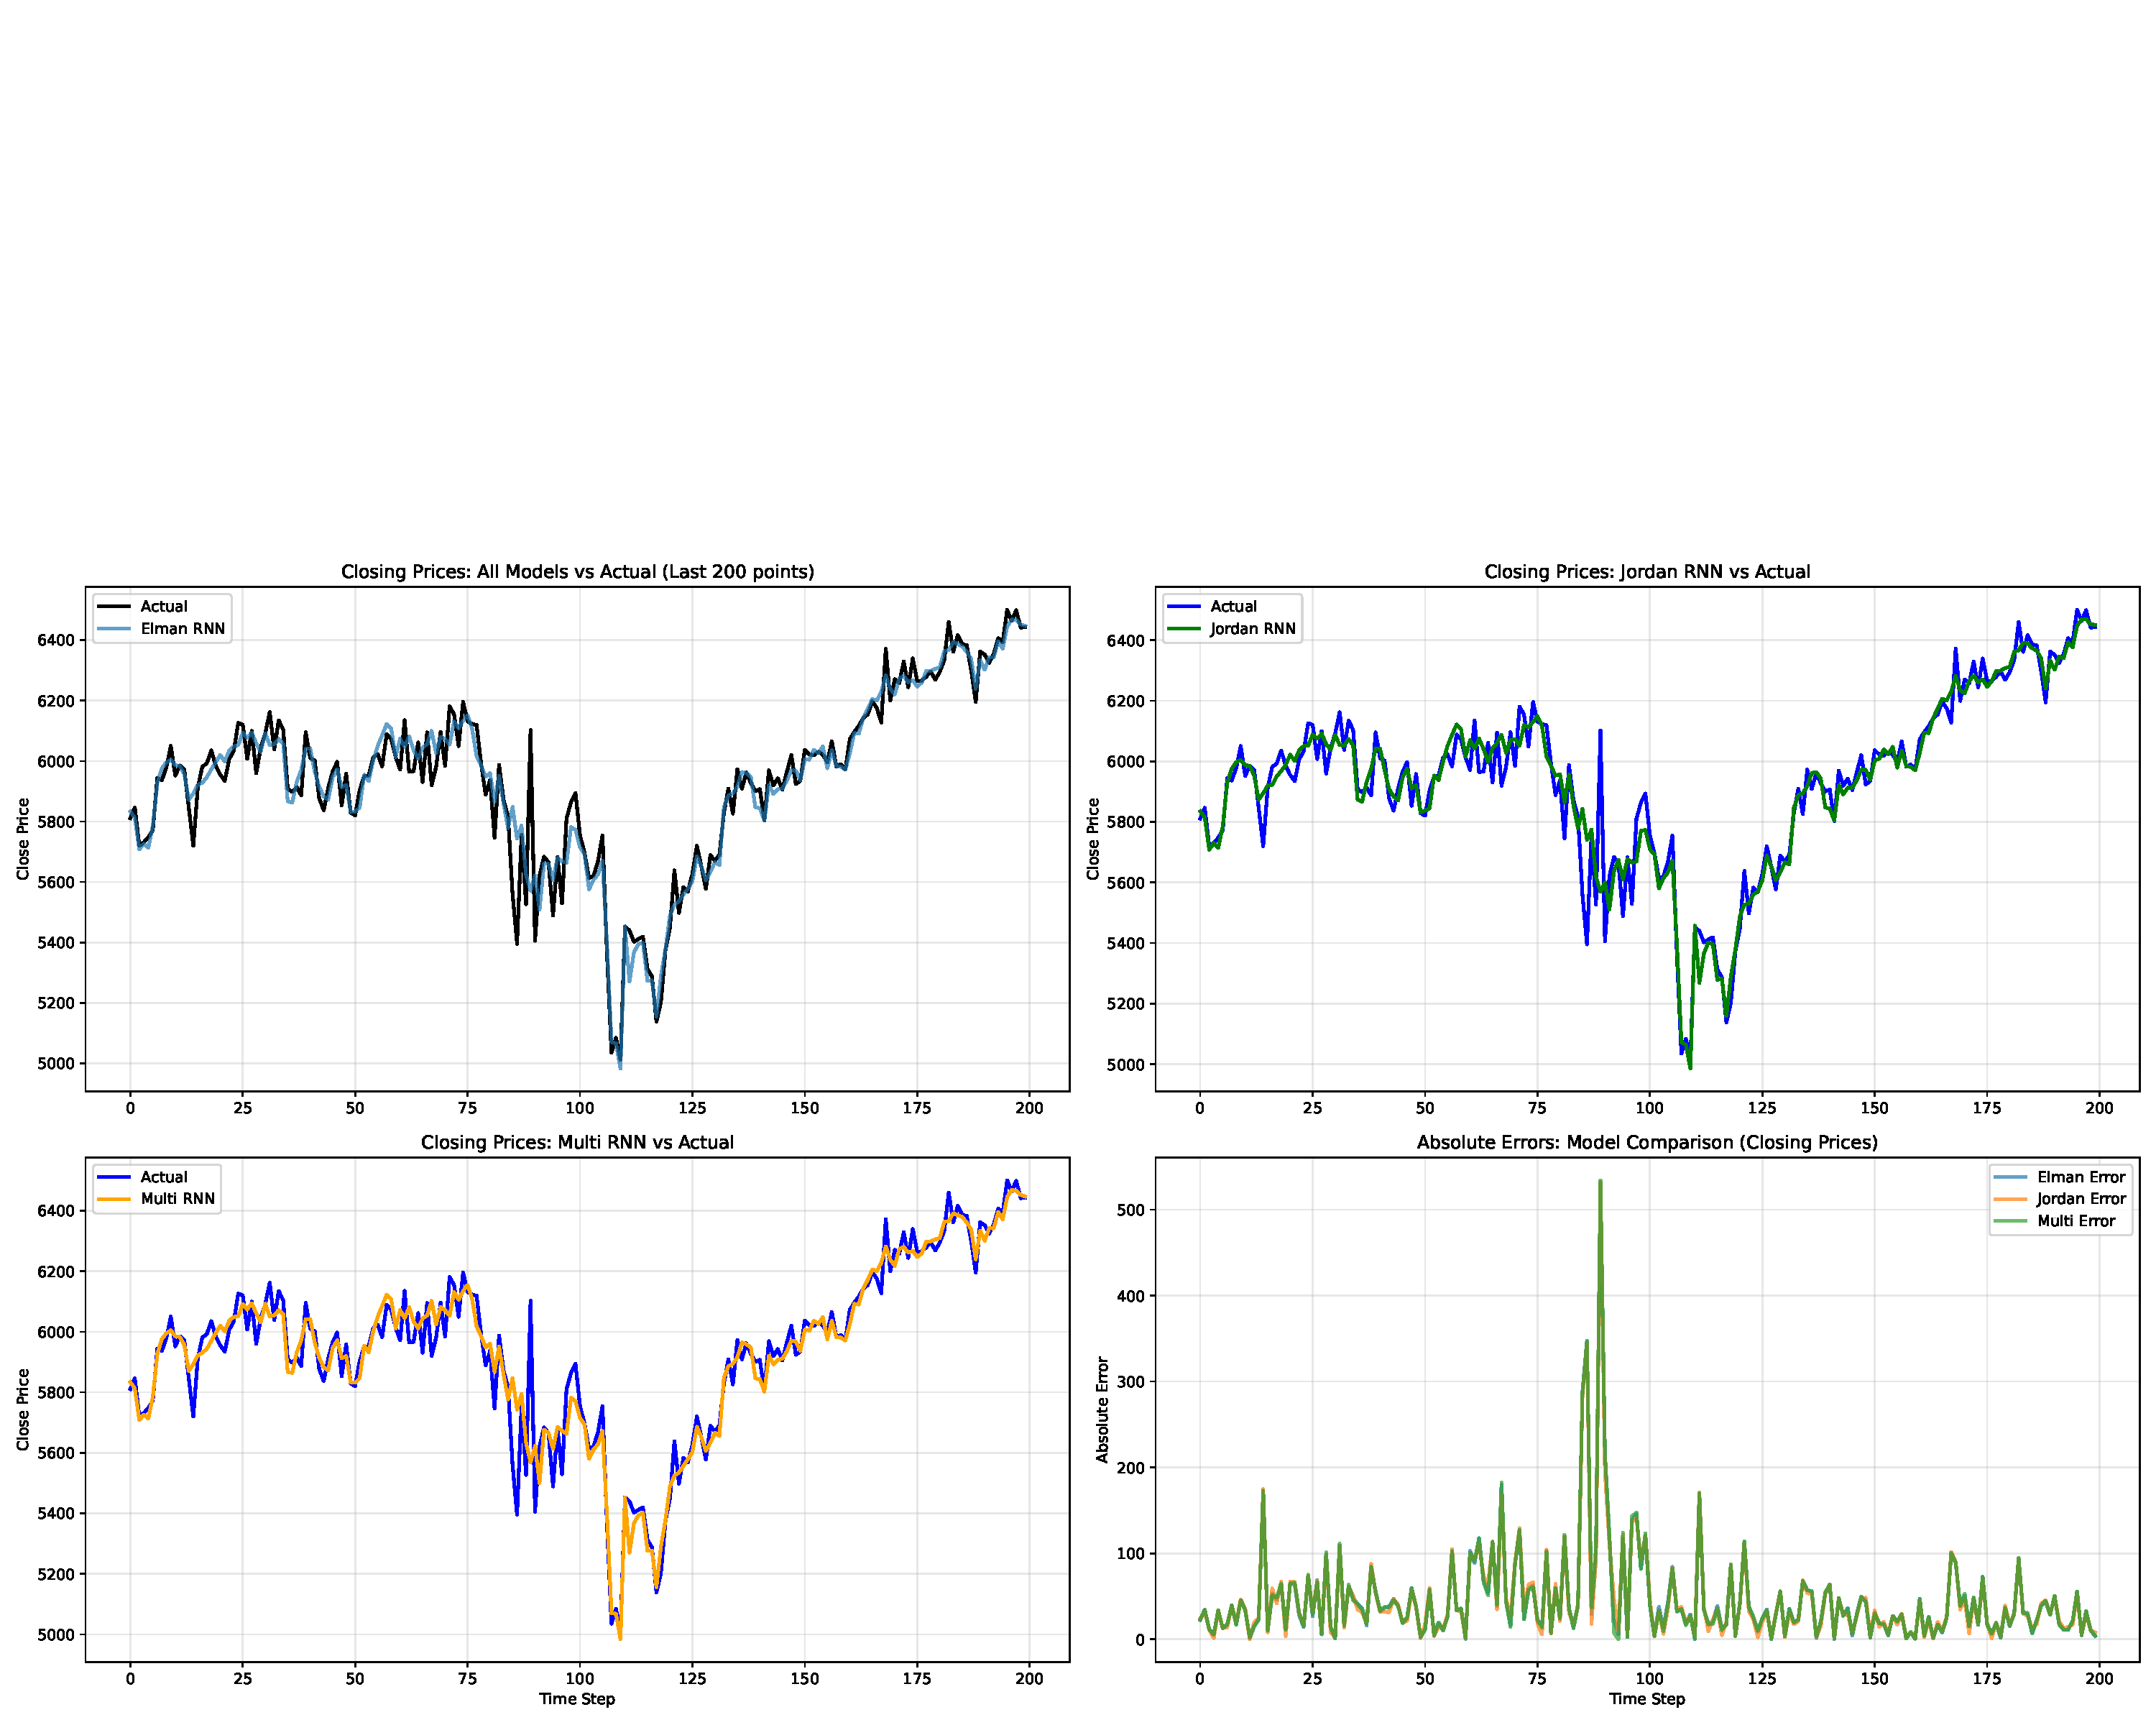
\includegraphics[width=0.5\textwidth]{plots/rnn_model_comparison_spy.pdf}
    \caption{S\$P500 Dataset plots}
    \label{fig:plots_spy}
\end{figure}

This result is consistent with the challenges of forecasting in efficient markets, where extracting a predictive signal
is notoriously difficult. The fact that no single architecture demonstrated a distinct advantage suggests they all faced
similar limitations in modeling the stochastic nature of stock returns.

% \subsection{Weather Dataset}
% TODO:
% \begin{table}[H]
%     \centering
%     \begin{tabular}{|l|c|c|c|c|}
%         \hline
%         \textbf{Model}& \textbf{RMSE} & \textbf{MAE} \\ 
%         \hline
%         Elman-RNN& todo & todo \\ 
%         \hline
%         Jordan-RNN & todo & todo \\ 
%         \hline
%         MRNN & todo & todo \\ 
%         \hline
%         \textbf{Best Model} & \multicolumn{2}{c|}{{todo}} \\ 
%         \hline
%     \end{tabular}
%     \vspace{4pt}
%     \caption{Performance Metrics for Weather Dataset}
%     \label{tab:results_wtr}
% \end{table}

\section{Conclusion}

This comparative study of the Elman-RNN, Jordan-RNN, and Multi-Recurrent Neural Network (MRNN) architectures for time
series forecasting across five diverse datasets reveals strikingly similar predictive performance among the models.
Despite their distinct feedback mechanisms like hidden state recurrence in Elman, output recurrence in Jordan, and a hybrid
approach in MRNN - no single architecture consistently outperformed the others in terms of RMSE and MAE on the holdout
test sets. The marginal differences observed, such as the Elman-RNN's slight edge on the electricity load data or the
Jordan-RNN's minor advantage on financial indices, were not significant enough to indicate a clear superiority. These
findings underscore that, for these RNN variants examined, the impact of architectural differences is minimal
when coupled with rigorous hyperparameter tuning, appropriate data preprocessing, and time-respecting cross-validation.
Future research could explore more complex RNN extensions or alternative neural architectures to potentially uncover
greater performance distinctions in time series forecasting tasks.

\bibliographystyle{IEEEtran}
\nocite{myrepo}
\bibliography{refs.bib}
% \pagebreak

\appendix
\section{Optimal Hyperparameters from Grid Search}

\begin{table}[H] 
    \centering 
    \resizebox{0.45\textwidth}{!}{ % Adjust 0.85 as needed
    \begin{tabular}{|l|c|c|c|} 
        \hline 
        \multicolumn{4}{|c|}{\textbf{Synthetic Autoregressive Stationary Dataset}} \\ \hline
        \textbf{Hyperparameter} & \textbf{Elman} & \textbf{Jordan} & \textbf{Multi} \\ 
        \hline 
        Hidden Size & 96 & 32 & 32 \\ 
        \hline
        Learning Rate & 1e-05 & 1e-05 & 1e-05 \\ 
        \hline
        Sequence Length & 10 & 10 & 10 \\ 
        \hline
        Weight Decay & 0.001 & 0.001 & 1e-05 \\ 
        \hline
        Patience & 10 & 10 & 10 \\ 
        \hline 
        
        \multicolumn{4}{|c|}{\textbf{CBOE VIX Daily OHLC Dataset}} \\ \hline
        \textbf{Hyperparameter} & \textbf{Elman} & \textbf{Jordan} & \textbf{Multi} \\ 
        \hline 
        Hidden Size & 64 & 32 & 64 \\ 
        \hline
        Learning Rate & 1e-05 & 1e-05 & 1e-05 \\ 
        \hline
        Sequence Length & 10 & 10 & 10 \\ 
        \hline
        Weight Decay & 0.0001 & 0.001 & 1e-05 \\ 
        \hline
        Patience & 10 & 10 & 10 \\ 
        \hline 
        
        \multicolumn{4}{|c|}{\textbf{ElectricityLoadDiagrams20112014 Dataset}} \\ \hline
        \textbf{Hyperparameter} & \textbf{Elman} & \textbf{Jordan} & \textbf{Multi} \\ 
        \hline 
        Hidden Size & 32 & 64 & 32 \\ 
        \hline
        Learning Rate & 0.0005 & 0.0001 & 0.0005 \\ 
        \hline
        Sequence Length & 10 & 10 & 10 \\ 
        \hline
        Weight Decay & 0.001 & 1e-05 & 0.001 \\ 
        \hline
        Patience & 10 & 10 & 10 \\ 
        \hline 
        
        \multicolumn{4}{|c|}{\textbf{S\&P 500 ETF Daily OHLCV Dataset}} \\ \hline
        \textbf{Hyperparameter} & \textbf{Elman} & \textbf{Jordan} & \textbf{Multi} \\ 
        \hline 
        Hidden Size & 32 & 32 & 32 \\ 
        \hline
        Learning Rate & 1e-05 & 1e-05 & 1e-05 \\ 
        \hline
        Sequence Length & 10 & 10 & 10 \\ 
        \hline
        Weight Decay & 0.0001 & 0.0001 & 0.0001 \\ 
        \hline
        Patience & 10 & 10 & 10 \\ 
        \hline 
        
        \multicolumn{4}{|c|}{\textbf{Weather Dataset}} \\ \hline
        \textbf{Hyperparameter} & \textbf{Elman} & \textbf{Jordan} & \textbf{Multi} \\ 
        \hline 
        Hidden Size & 32 & 64 & 64 \\ 
        \hline
        Learning Rate & 0.0005 & 0.0001 & 0.0005 \\ 
        \hline
        Sequence Length & 10 & 10 & 10 \\ 
        \hline
        Weight Decay & 0.001 & 1e-05 & 0.001 \\ 
        \hline
        Patience & 10 & 10 & 10 \\ 
        \hline 
    \end{tabular}
    }
    \vspace{12pt}
    \caption{Optimal hyperparameter values for Elman, Jordan, and Multi RNN models across five datasets.} 
    \label{hyperparameters}
\end{table}





\end{document}